%%%%%%%%%%%%  Generated using docx2latex.com  %%%%%%%%%%%%%%

%%%%%%%%%%%%  v2.0.0-beta  %%%%%%%%%%%%%%

\documentclass[12pt]{report}
\usepackage{amsmath}
\usepackage{latexsym}
\usepackage{amsfonts}
\usepackage[normalem]{ulem}
\usepackage{soul}
\usepackage{array}
\usepackage{amssymb}
\usepackage{extarrows}
\usepackage{graphicx}
\usepackage[backend=biber,
style=numeric,
sorting=none,
isbn=false,
doi=false,
url=false,
]{biblatex}\addbibresource{bibliography.bib}

\usepackage{subfig}
\usepackage{wrapfig}
\usepackage{wasysym}
\usepackage{enumitem}
\usepackage{adjustbox}
\usepackage{ragged2e}
\usepackage[svgnames,table]{xcolor}
\usepackage{tikz}
\usepackage{longtable}
\usepackage{changepage}
\usepackage{setspace}
\usepackage{hhline}
\usepackage{multicol}
\usepackage{tabto}
\usepackage{float}
\usepackage{multirow}
\usepackage{makecell}
\usepackage{fancyhdr}
\usepackage[toc,page]{appendix}
\usepackage[hidelinks]{hyperref}
\usetikzlibrary{shapes.symbols,shapes.geometric,shadows,arrows.meta}
\tikzset{>={Latex[width=1.5mm,length=2mm]}}
\usepackage{flowchart}\usepackage[paperheight=11.69in,paperwidth=8.27in,left=1.0in,right=1.0in,top=1.0in,bottom=1.0in,headheight=1in]{geometry}
\usepackage[utf8]{inputenc}
\usepackage[T1]{fontenc}
\TabPositions{0.5in,1.0in,1.5in,2.0in,2.5in,3.0in,3.5in,4.0in,4.5in,5.0in,5.5in,6.0in,}

\urlstyle{same}


 %%%%%%%%%%%%  Set Depths for Sections  %%%%%%%%%%%%%%

% 1) Section
% 1.1) SubSection
% 1.1.1) SubSubSection
% 1.1.1.1) Paragraph
% 1.1.1.1.1) Subparagraph


\setcounter{tocdepth}{5}
\setcounter{secnumdepth}{5}


 %%%%%%%%%%%%  Set Depths for Nested Lists created by \begin{enumerate}  %%%%%%%%%%%%%%


\setlistdepth{9}
\renewlist{enumerate}{enumerate}{9}
		\setlist[enumerate,1]{label=\arabic*)}
		\setlist[enumerate,2]{label=\alph*)}
		\setlist[enumerate,3]{label=(\roman*)}
		\setlist[enumerate,4]{label=(\arabic*)}
		\setlist[enumerate,5]{label=(\Alph*)}
		\setlist[enumerate,6]{label=(\Roman*)}
		\setlist[enumerate,7]{label=\arabic*}
		\setlist[enumerate,8]{label=\alph*}
		\setlist[enumerate,9]{label=\roman*}

\renewlist{itemize}{itemize}{9}
		\setlist[itemize]{label=$\cdot$}
		\setlist[itemize,1]{label=\textbullet}
		\setlist[itemize,2]{label=$\circ$}
		\setlist[itemize,3]{label=$\ast$}
		\setlist[itemize,4]{label=$\dagger$}
		\setlist[itemize,5]{label=$\triangleright$}
		\setlist[itemize,6]{label=$\bigstar$}
		\setlist[itemize,7]{label=$\blacklozenge$}
		\setlist[itemize,8]{label=$\prime$}



 %%%%%%%%%%%%  Header here  %%%%%%%%%%%%%%


\pagestyle{fancy}
\fancyhf{}
\cfoot{ 
\vspace{\baselineskip}
}
\renewcommand{\headrulewidth}{0pt}
\setlength{\topsep}{0pt}\setlength{\parskip}{8.04pt}
\setlength{\parindent}{0pt}

 %%%%%%%%%%%%  This sets linespacing (verticle gap between Lines) Default=1 %%%%%%%%%%%%%%


\renewcommand{\arraystretch}{1.3}


%%%%%%%%%%%%%%%%%%%% Document code starts here %%%%%%%%%%%%%%%%%%%%



\begin{document}
\begin{Center}
B. Tech. – Project
\end{Center}\par

\begin{Center}
On
\end{Center}\par

\begin{Center}
Flexible Endoscopic Robot
\end{Center}\par

\begin{Center}
(Project code: D8)
\end{Center}\par


\vspace{\baselineskip}
\begin{Center}
Submitted by:
\end{Center}\par

\begin{Center}
Kshitij Gupta (Entry No: 2016ME20760)
\end{Center}\par

\begin{Center}
Shantnav Agarwal (Entry No: 2016ME20767)
\end{Center}\par


\vspace{\baselineskip}
\begin{Center}
Supervised by:
\end{Center}\par

\begin{Center}
Professor Jitendra Prasad Khatait
\end{Center}\par



%%%%%%%%%%%%%%%%%%%% Figure/Image No: 1 starts here %%%%%%%%%%%%%%%%%%%%

\begin{figure}[H]
	\begin{Center}
		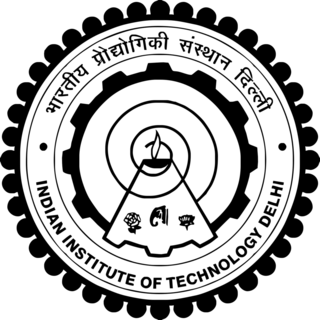
\includegraphics[width=3.33in,height=3.33in]{./media/image1.png}
	\end{Center}
\end{figure}


%%%%%%%%%%%%%%%%%%%% Figure/Image No: 1 Ends here %%%%%%%%%%%%%%%%%%%%

\par


\vspace{\baselineskip}
\begin{Center}
Mechanical Engineering Department
\end{Center}\par

\begin{Center}
Indian Institute of Technology Delhi
\end{Center}\par

\begin{Center}
November 2019
\end{Center}\par



 %%%%%%%%%%%%  Starting New Page here %%%%%%%%%%%%%%

\newpage

\vspace{\baselineskip}\begin{Center}
{\fontsize{16pt}{19.2pt}\selectfont Acknowledgement\par}
\end{Center}\par

We would like to express sincere gratitude to our supervisor Prof. J P Khatait for his continued support. He always made time out of his busy schedule and his consistent guidance and valuable advises really helped us achieve results.\par


\vspace{\baselineskip}
\begin{Center}
{\fontsize{16pt}{19.2pt}\selectfont Abstract\par}
\end{Center}\par

A simulation of the navigation of an endoscopic device inside a human body has been attempted on SPACAR. We have made use of Finite Element based approach to model the instrument and the colon. The colon is modelled by a centreline comprising 2-dimensional (planar) beam elements and the contact forces are based on the Hertzian contact model. The endoscope has also been modelled as multiple finite planar beam elements for optimally calculating the deformation and forces endured during operation.\par

A simple dynamic force field approach has been developed to mimic the contact behaviours between the colon and the instrument. We have approximated adequate parameters for beam bending and longitudinal stiffness using available mechanical properties in order to develop a realistic model of the colon. Friction and damping forces have been incorporated as well and the coefficients pertaining to human tissue have been chosen for our purpose.\par



 %%%%%%%%%%%%  Starting New Page here %%%%%%%%%%%%%%

\newpage

\vspace{\baselineskip}

 %%%%%%%%%%%%  This Produces Table Of Contents %%%%%%%%%%%%%%

\tableofcontents
\addcontentsline{toc}{chapter}{Contents}
\listoffigures
\addcontentsline{toc}{chapter}{List of Figures}
\listoftables
\addcontentsline{toc}{chapter}{List of Tables}


%%%%%%%%%%%%%%%%%%%% Table No: 1 starts here %%%%%%%%%%%%%%%%%%%%


\begin{table}[H]
 			\centering
\begin{tabular}{p{3.09in}p{3.09in}}
%row no:1
\multicolumn{1}{p{3.09in}}{Index of Tables \par  \par  \par  \par  \tabto{6.26in} } & 
\multicolumn{1}{p{3.09in}}{Index of Figures \par  \par  \par  \par  \par \href{https://csciitd-my.sharepoint.com/personal/me2160767_csciitd_onmicrosoft_com/Documents/Semesters/Semester%207/BTP/BTP%20mid-term%20report.docx}{Figure 5: Planar beam element \tabto{6.26in} 13} \par  \par \href{https://csciitd-my.sharepoint.com/personal/me2160767_csciitd_onmicrosoft_com/Documents/Semesters/Semester%207/BTP/BTP%20mid-term%20report.docx}{Figure 7: Diagram to explain the algorithm \tabto{6.26in} 20} \par  \par \href{https://csciitd-my.sharepoint.com/personal/me2160767_csciitd_onmicrosoft_com/Documents/Semesters/Semester%207/BTP/BTP%20mid-term%20report.docx}{Figure 9: Scaled diagram of large diagram \tabto{6.26in} 22} \par  \par  \par } \\
\hhline{~~}

\end{tabular}
 \end{table}


%%%%%%%%%%%%%%%%%%%% Table No: 1 ends here %%%%%%%%%%%%%%%%%%%%



 %%%%%%%%%%%%  Starting New Page here %%%%%%%%%%%%%%

\newpage

\vspace{\baselineskip}\section*{Introduction}
\addcontentsline{toc}{section}{Introduction}
Modern surgery has progressed rapidly with advancement\ in\ technology and medication.  Earlier, treating or observing any internal part of the body required a surgeon to make large incisions resulting in excessive blood loss, pain, infection and a longer recovery period.  The introduction of Minimally-Invasive-Surgery in recent years had greatly reduced damage to tissues leading to faster recovery. Natural Orifice Transluminal Endoscopic Surgery (NOTES), which involves accessing organs through natural orifices, is one of the most important development in the field. Further advancements to this field in terms of endoscopes now give rise to the possibility of observing and treating diseases with almost no blood loss and damage to the tissue. \par

These endoscopic instruments allow the surgeon to deploy cameras to observe the intestine of the patient and check for ulcers, tumours, inflammation etc; they can be used to place the ultrasound probe closer to organs that can be difficult to image, such as pancreas; finally, endoscopes can also be used to carry out surgery such as removal of gallbladder, sealing/ tying fallopian tubes and removal of tumours.\par

Among all types of endoscopy, colonoscopy is extensively used, with over 3 crore operations per year. However, it requires highly skilled and professionally trained surgeons. The process is often painful, particularly due to high force exerted on the walls of the colon when the examiner pushes the instrument inward. The colon wall is twisted and is highly folded; the tip control, therefore, is very challenging and the practitioner often needs to readjust for the overshoot. Applying too much pressure to change the manoeuvre the instrument can rupture the wall, which may have fatal consequences. In many cases, the cecum, i.e. other end of the intestine, is not reached and these incomplete inspections lead to high polyp miss rate (cancer would go undetected).\par



%%%%%%%%%%%%%%%%%%%% Figure/Image No: 2 starts here %%%%%%%%%%%%%%%%%%%%

\begin{figure}[H]
	\begin{Center}
		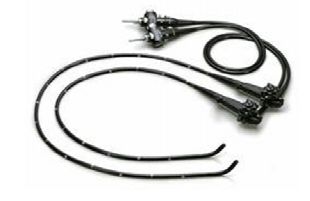
\includegraphics[width=2.31in,height=1.0in]{./media/image2.png}
		\caption{: Commercial colonoscope}
		\label{fig:_Commercial_colonoscope}
	\end{Center}
\end{figure}


%%%%%%%%%%%%%%%%%%%% Figure/Image No: 2 Ends here %%%%%%%%%%%%%%%%%%%%

\par

\par

The use of robotics systems in colonoscopy allows for more precision, miniaturization and smaller incisions. Further, these robotic systems allow the surgeon to control instruments in a more convenient working position, it scales his movements and improve visualisation by showing enhanced three-dimensional magnified images. Naturally occurring tremors are filtered out by the robot automatically decreasing chances of human error.\par

In our project we want to focus our attention on the interaction between multiple soft bodies allowing us to simulate the movement of a soft robotic endoscope/ colonoscope inside a human body. Just like the current medical procedures where the doctor is physically controlling only one end of the endoscope, we are also constraining the translational and rotational motion of only one end of the device. Through this exercise, we aim to find the push forces and the suitable material properties that can be used for the endoscopic tube.\par

An accurate modelling of the characteristics of the motion of a robot inside the human body is critical for further development of these robots as well as proper training of medical professionals. Modelling these interactions however is extremely complex and challenging. Machado et. al. \cite{MACHADO201299} talk about how geometry, kinematics and nature of the contacting body all play a critical role in determining the stiffness and damping coefficient of the contact. Further, non-smooth systems also exhibit nonlinearities and discontinuities such as those caused by intermittent contact, nonlinear material properties etc. \par

For the contact model, we have used Hertz contact forces wherein we ignore energy transfer and focus on linear elastic bodies. We have made use of multiple planar finite beam elements to represent the endoscopic tube and the colon while surrounding part of the colon centreline has been defined as force fields. A simple dynamic force field approach has been developed to mimic the contact behaviours between the colon and the instrument. We have determined the beam bending and longitudinal stiffness using available mechanical properties in order to develop a realistic model of the colon.\par

Rest of the report is divided in six chapters (chapter 2 through 7). Chapter 2 gives some background on the simple soft body contact force models that are in common use. It then reviews the force modelling that has been done in recent in the field of endoscopy and catheters and particularly focusses on the software modelling of the navigation. Chapter 3 gives the detailed problem description and the general objectives of this study. Subsequent chapters are the detailed description of the work done, starting from Chapter 4 which provides a brief theory involved in the project. The next chapter describes the work done in progressive stages, including the development of the dynamic force field approach and the finite element model. Chapter 6 gives a brief of the simulations and results, followed by the last chapter which gives the final conclusions.\par

\section*{Literature Survey}
\addcontentsline{toc}{section}{Literature Survey}
Over the last few decades, several contact models have been proposed, most of which have the Hertzian model as their foundation. The classical Hertzian theory states that contact force is a nonlinear function of the depth of indentation, assuming the bodies are perfectly elastic and there is no energy dissipation. However, this model has many limitations and is not suited for any practical application. Machado, et al.\cite{MACHADO201299} in \textit{Compliant contact force models in multibody dynamics} describe various compliant force, i.e. based on indentation and contacting bodies' properties, formulations which try to deal with the problems associated with the Hertzian model. Two widely used models are Kelvin Voigt model which includes a damping term which is dependent on contact velocity and Lankarani-Nikravesh model which accounts for permanent deformations using a hysteresis damping coefficient. Kelvin Voigt model too has a serious drawback, i.e., the force at the beginning of the contact is not zero due to a non-zero velocity term. Continuous contact forces for soft bodies have been comprehensively described in a review paper by Paulo Flores\cite{Flores2011}, et al. who gives an overview of three approaches: \par

\begin{enumerate}
	\item Dissipation with coefficient of restitution involving balance of energies and momentum.\par

	\item Storage of a part of kinetic energy as elastic energy which would lead to deformations. \par

	\item Dissipation through internal damping.
\end{enumerate}\par

Most of the work being done in endoscopy nowadays focus on either creating physical models or simulations using computer graphics and virtual reality for the training of the practitioners. There are numerous papers like Tingxi Wen et al.\cite{Wen2018} and MacIntosh et al.\cite{mcintoshComputerbasedVirtualReality2014} which focus purely on virtual reality training based on a real-time computational approach.\par

Woojin Ahn, et al.\cite{1571560} describe a contact model which calculates forces given displacement measurements by a virtual reality-based colonoscopy simulator. Levin J. Sliker et al.\cite{SLIKER2016472} present a frictional resistance model for tissue-capsule endoscope sliding contact. The model outputs the drag force required to move the endoscopic capsule through the gastrointestinal tract. However, this model is limited to interaction between a stiff small capsule and incompressible tissue.  Many authors have also attempted to develop friction models based on Lankarani-Nikravesh forces.\par

Some work has also been done on simulation-based in relatively more conventional settings. Alexander Verl in his book, \textit{Soft Robotics: Transferring theory to Applications}, describes some state-of-the-art simulation techniques for soft body robotics and the basic concepts of e-Robotics, which provides a comprehensive software environment suited for such applications. Khatait et al.\cite{inproceedings} use a simulation software \textit{SPACAR }to model the sliding contact forces of a flexible endoscope inside a comparatively rigid tube. The rigid tube is described with multiple beam elements whereas the tube is essentially a force field in a 3-D Bezier curve form. The endoscope is held at its rear end where no rotation is allowed and as the instrument enters the tube, it experiences a force depending on the contact penetration and damping coefficient of the tube wall. The force field is a slight variant of Kelvin Voigt contact model and is divided into two regions: \par

\begin{enumerate}
	\item Transition region, where the indentation term is a second-order polynomial and the damping term is third order.\par

	\item Full contact region with linear polynomials. \par

	\item A simple friction term is also incorporated in the given approach. 
\end{enumerate}\par



%%%%%%%%%%%%%%%%%%%% Figure/Image No: 3 starts here %%%%%%%%%%%%%%%%%%%%

\begin{figure}[H]
	\begin{Center}
		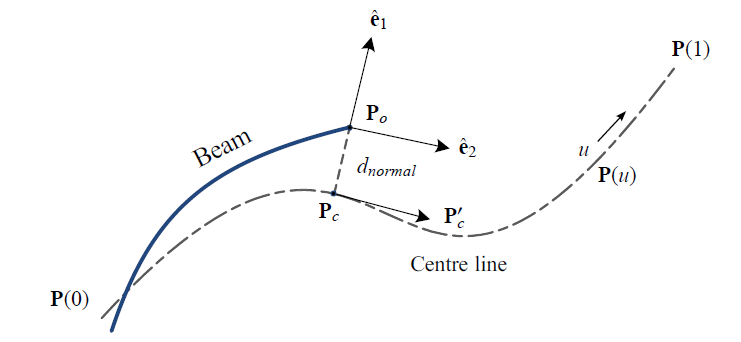
\includegraphics[width=5.11in,height=2.66in]{./media/image3.png}
		\caption{: Simulation of forces using Bezier curves}
		\label{fig:_Simulation_of_forces_using_Bezier_curves}
	\end{Center}
\end{figure}


%%%%%%%%%%%%%%%%%%%% Figure/Image No: 3 Ends here %%%%%%%%%%%%%%%%%%%%

\par

\par

Charles R. Welch and John D Reid did colonoscopy simulations in a slightly more sophisticated software LS-DYNA. The tissues here are modelled through adjusted Mooney-Rivlin rubber model and the results are obtained for different parameters iteratively. The simulation attempts to show the looping phenomenon, a phenomenon in which the endoscope forms a loop along the walls of the colon due to the application of larger forces which leads to more difficulty in manoeuvring and poses a significant challenge to overcome for the doctor.\par

Perhaps much more work in navigation has been done in catheters than colonoscopy. Catheters are thin tubes (similar to endoscopes) which are inserted in the body to treat disease or perform surgery. In the simplest use, they are used to empty the bladder, but henceforth only the cardiovascular catheters which are inserted through the veins are discussed. In one of the earliest developments by M. Negoro et al.\cite{Negoro2001AnIC}, the interventionalist (surgeon) uses a joystick to advance the catheter using the push, pull, and rotate technique, although this system is now largely being replaced by remote magnetic controllers. The controller as a slave device has 2-axis force sensor, which measures the contact force between blood vessels and the catheter. There is a micro force sensor in the tip of the catheter, which measures the contact force between the catheter tip and the blood vessel wall. The influences of forces on its navigation has thus been studied extensively.\par

MATLAB simulation of contact forces has been attempted by Wang et al.\cite{6885827} in which they propose push-based passive catheter control model. The classical models in catheter navigation are position-based, but the tip motion in this case is not smooth and continuous. The simulation shows relatively smoother motion in case of the model proposed here. Push force, catheter length and the parameters of the blood vessel are the input to the simulation model and the position of the catheter tip is calculated using piecewise constant curvature technique. Using the information of the catheter, the safety threshold of the push force can be calculated.\par



%%%%%%%%%%%%%%%%%%%% Figure/Image No: 4 starts here %%%%%%%%%%%%%%%%%%%%

\begin{figure}[H]
	\begin{Center}
		\includegraphics[width=5.73in,height=3.59in]{./media/image4.gif}
		\caption{: Simulation of forces using constant curvature continuum robot}
		\label{fig:_Simulation_of_forces_using_constant_curvature_continuum_robot}
	\end{Center}
\end{figure}


%%%%%%%%%%%%%%%%%%%% Figure/Image No: 4 Ends here %%%%%%%%%%%%%%%%%%%%

\par

\par

This continuum robot approach is different from the discrete finite element approach that is discussed in this report. A continuum robot can be defined as a continuously bending, infinite-degree of-freedom robot with an elastic structure. More specifically, Wang et al. uses piecewise constant curvature continuum model described by a finite set of arc parameters. The mathematics of such model is simple and is described in a review paper by Webster et al.\cite{doi:10.1177/0278364910368147}\par

In his thesis, Tehnikateaduste Magistri\cite{Mag12} has attempted to model the colon using finite beam elements using MATLAB. The behaviour of the wall is non-linear, and folds have been added in the model as well. The two walls of the intestine are connected using virtual connection elements (springs).\par


\vspace{\baselineskip}


%%%%%%%%%%%%%%%%%%%% Figure/Image No: 5 starts here %%%%%%%%%%%%%%%%%%%%

\begin{figure}[H]
	\begin{Center}
		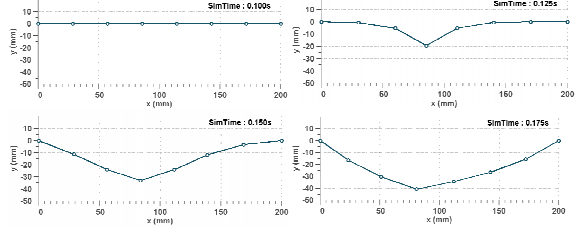
\includegraphics[width=6.1in,height=2.43in]{./media/image5.png}
		\caption{: Verification of the FE colon model}
		\label{fig:_Verification_of_the_FE_colon_model}
	\end{Center}
\end{figure}


%%%%%%%%%%%%%%%%%%%% Figure/Image No: 5 Ends here %%%%%%%%%%%%%%%%%%%%

\par

\par

The normal contact forces in this case are calculated using penalty approach in Simulink. Verification was done by poking the model of the colon in the perpendicular direction and comparing the forces from the model with the observed value.\par



 %%%%%%%%%%%%  Starting New Page here %%%%%%%%%%%%%%

\newpage

\vspace{\baselineskip}\section*{Project Objectives and Work Plan}
\addcontentsline{toc}{section}{Project Objectives and Work Plan}
\subsection*{Motivation}
\addcontentsline{toc}{subsection}{Motivation}
Modern day endoscopic operations entail a lot of problems; even the most experienced surgeons find it difficult to navigate inside the complex structures of the body or to avoid the chances of loop formation. The problem in hand is to accurately simulate the navigation of a flexible endoscopic robot using multielement formulation. This not only involves modelling the motion of the endoscope but also suitably defining the interacting environment. The simulation shall enable us to study the forces involved in endoscopic surgeries and their effect on the motion of the front tip and if possible, the phenomenon of looping. Further these simulations can be used to train surgeons as well.\par

However, to accurately model and verify these simulations is extremely difficult because it is almost impossible to obtain any real-world data. Fan etal. \cite{fanTwolayeredMechanicalModel2004} do talk about carrying out tests on rats, however doing such a detailed study is beyond the scope of this paper. We aim to develop and perfect simulations of interaction of beam elements with various simple shapes and build further on that. We have talked about this in more detail in the section 4.2.\par

In our B. Tech project, we set out with the goal of analytically simulating the interaction of deformable bodies. This has, to some extent, already been achieved by using Finite Element Analysis in software such as LS-Dyna. However, FEA is computationally very expensive and requires complex modelling of all the bodies involved. \par

Through our project, we have developed a simpler interface in which the user can enter the shape of the bodies taking part in the interaction as (x, y) coordinates, define the parameters of Hertzian contact model, and enter the physical properties of the bodies involved. From there our model will take over and simulate the interaction between the two bodies. \par

\subsection*{Objectives Achieved}
\addcontentsline{toc}{subsection}{Objectives Achieved}
\begin{enumerate}
	\item Simulate the navigation of a flexible endoscope inside a human large intestine using a simulation software. The interaction between the soft bodies will be broadly based on Hertzian contact force models. We have selected a force formulation which will appropriately model the effect of wall damping and hysteresis and consider the frictional forces involved. \par

	\item Model the human large intestine using simple geometries where forces are defined as force fields around a deformable beam element. These fields accurately model the nonlinearity in the stiffness and damping properties of the walls. As the beam element defining the human large intestine deforms, the fields also dynamically change their shape to conform to the new shape of the large intestine geometry.\par

	\item The endoscope is also modelled as multiple beam elements. By using analytical formulation, we can focus our computation on the deformation of the endoscope while closely mimicking actual forces acting upon it.\par

	\item Observed the forces, deformation and stress endured by the endoscope during the procedure. This shall allow us to ascertain the range of suitable material properties for a soft surgical robot.
\end{enumerate}\par

\subsection*{Methodology}
\addcontentsline{toc}{subsection}{Methodology}
To achieve our objectives, we had to\par

\begin{enumerate}
	\item Model the endoscope as well as the human large intestine as combination of multiple beam elements.\par

	\item Model the force fields around all beam elements of the human large intestine. Since with each time step, the beam elements deform, the force fields are also constantly changing. This has been discussed further in Section 4 in more detail.\par

	\item Develop simple simulation instances to ensure that the behaviour of beam element of the large intestine is like the large intestine’s behaviour in real life.\par

	\item To carry out our simulations, we are making use of the software SPACAR. SPACAR is based on the non-linear finite element theory and is well suited for the analysis of rigid and flexible structures in both 2-D and 3-D environments. It is computationally efficient and allows for a detailed visualisation of the endoscope in the environment using tools like SPAVISUAL.
\end{enumerate}\par



 %%%%%%%%%%%%  Starting New Page here %%%%%%%%%%%%%%

\newpage

\vspace{\baselineskip}\section*{Theory}
\addcontentsline{toc}{section}{Theory}
The relevant theory is described in following two sections: 4.1.1. FEA of the endoscope (made of beam elements), 4.1.2. Contact force fields\par

\subsection*{Endoscope}
\addcontentsline{toc}{subsection}{Endoscope}
The endoscope is made up of planar beam elements which are already defined in the simulation software SPACAR. A 2-D flexible beam element has two nodes and 6 degrees of freedom. It is therefore defined by x and y coordinates of the two nodes and the angle of rotation at the two nodes. JB Jonker in his book Dynamics of Machine\cite{JBJ09} defines the flexibility of the beam element in terms of three ‘deformation modes’ (\textbf{e}). The first deformation mode represents the elongation in the beam, while the other two capture the bending angle at the two ends. The deformation modes can thus be defined as follows:\par


\vspace{\baselineskip}


%%%%%%%%%%%%%%%%%%%% Figure/Image No: 6 starts here %%%%%%%%%%%%%%%%%%%%

\begin{figure}[H]
	\begin{FlushLeft}		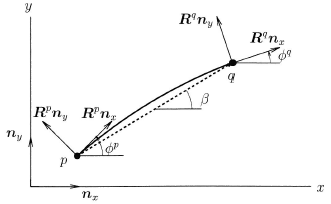
\includegraphics[width=3.45in,height=2.12in]{./media/image6.png}
	\end{FlushLeft}\end{figure}


%%%%%%%%%%%%%%%%%%%% Figure/Image No: 6 Ends here %%%%%%%%%%%%%%%%%%%%

\begin{FlushLeft}
e\textsubscript{1} = l-l\textsubscript{0} (elongation)\ \  \ \ \ \ \ \ \ \ \ \ \ \ \ \ \ \ \ \ \  (i)
\end{FlushLeft}\par

\begin{FlushLeft}
e\textsubscript{2} = -(\textbf{R}\textsuperscript{p}\textbf{n}\textsubscript{y}, l) (bending at end 1)\ \  (ii)
\end{FlushLeft}\par

\begin{FlushLeft}
(=(x\textsuperscript{q}-x\textsuperscript{p}) \( ~sin \varnothing ^{p} \)  - (y\textsuperscript{q}-y\textsuperscript{p}) \( ~cos \varnothing ^{p} \) )\ \  (iii)
\end{FlushLeft}\par

\begin{FlushLeft}
e\textsubscript{3} = (\textbf{R}\textsuperscript{q}\textbf{n}\textsubscript{y}, l) (bending at end 2)
\end{FlushLeft}\par

Here, l is the length of the beam element, l\textsubscript{0} the initial length, R\textsuperscript{p} and R\textsuperscript{q} are the rotation matrices at the two ends, i.e,\par

\par 
 \begin{tikzpicture}


% Error occured here... ignoring it.
\begin{adjustwidth}{3.5in}{0.0in}
\textbf{R}\textsuperscript{p} =  \(  \left[ \begin{matrix}
\cos \varnothing ^{p}  &  -sin \varnothing ^{p}\\
\sin \varnothing ^{p}  &  \cos \varnothing ^{p}\\
\end{matrix}
 \right]  \) \end{adjustwidth}


\end{tikzpicture}
\begin{adjustwidth}{3.5in}{0.0in}
\textbf{R}\textsuperscript{p}\textbf{n}\textsubscript{y} represents the vector perpendicular to the end ‘p’.\par

\end{adjustwidth}

After defining the beam elements, its inertial properties and external forces/ velocities, the software handles the kinematic and dynamic analysis part. A node or a deformation mode can be either independent (\textbf{x}\textsuperscript{m}, prescribed dof), dependent (\textbf{x}\textsuperscript{c}) or fixed (\textbf{x}\textsuperscript{o}). For the kinematic analysis part, each deformation mode \textbf{e} is written as a function (\textbf{\textit{D}}) of x (the expression for planar beam is given in (iii)).\  In a nutshell, \textbf{x} and \textbf{e} of the element are defined in terms of the generalised coordinates \textbf{q}, i.e. the complete motion is described with respect to the motion of the independent coordinates \textbf{x}\textsuperscript{m} through functions called geometric transfer functions (\textbf{\textit{F}}) and their derivatives are taken to calculate the velocities and accelerations. For dynamic analysis, the software uses the principle of virtual power and the principle of d’Alembert. Further discussion on kinematics and dynamics is beyond the scope of the report.\par

\subsection*{Contact Forces}
\addcontentsline{toc}{subsection}{Contact Forces}
To revisit and formalise some of the concepts discussed in Section 2, Hertzian contact forces are given by:\par

 \[ F=K \delta ^{n} \] \par

where K is the contact stiffness parameter and n is the nonlinear coefficient,  \(  \delta  \)  is the depth of indentation. \par

The Kelvin-Voigt model is an improvised model which considers damping forces proportional to the indentation speed. It is given by:\par

\begin{Center}
\textit{F}{\fontsize{8pt}{9.6pt}\selectfont \textit{N \par}}= \textit{K$ \delta $  }+\textit{D \( \dot{ \delta } \) }
\end{Center}\par

Where D is the damping coefficient and  \( \dot{ \delta } \)  is the velocity/ rate of indentation.\par

As was mentioned, these models suffer from some major issues and are not in much use. It was further refined by Lankarani-Nikravesh\cite{Lankarani1994} who included hysteresis damping coefficient: \par

 \[  \]  \[ F_{N}=K \delta ^{n} \left[ 1+ \frac{3 \left( 1-c_{r}^{2} \right) \dot{ \delta }}{4~\dot{ \delta ^{ \left( - \right) }}} \right]  \] \par

Here, c\textsubscript{r} is the coefficient of restitution and  \( \dot{ \delta ^{ \left( - \right) }} \)  is the relative approach velocity.\par

As can be seen, there is no damping for perfectly elastic system (c\textsubscript{r} = 0). The damping coefficient is written as D =  \(  \mu  \delta ^{n} \) , since damping\ should be zero for zero indentation (unlike Kelvin-Voigt model).  This equation is obtained by equating kinetic energy losses to the work done by the deformation forces. Work done is described as a hysteresis loop, i.e., \par

 \[  \]  \[  \oint _{}^{}D\dot{ \delta } d \delta = 2 \int _{0}^{ \delta _{m}} \mu  \delta ^{n}\dot{ \delta } d \delta  \] \par

The change in kinetic energy is simply:\par

 \[ \frac{1}{2}m^{eff}\dot{ \delta ^{ \left( - \right) }} \left( 1-c_{r}^{2} \right)  \] \par

Where m\textsuperscript{eff} is the effective mass of the system.\par

\subsection*{Assumptions}
\addcontentsline{toc}{subsection}{Assumptions}
There are several assumptions involved in our modelling:\par

\begin{enumerate}
	\item The endoscope and intestine have been assumed to be composed of planar beam elements; other way to model is continuum robotics analysis, which is more analytical. In our case, the forces are applicable (and the interaction is between) only the nodes of the two entities involved. There is a limitation on the number of nodes we can use.\par

	\item We have used Hertzian forces to model the contact; this is a very big assumption and a limitation as well. Hertzian forces and even the derived models like Lankarani-Nikravesh cannot sufficiently model large deformations. For these modelling, there is no closed form formula that can be used, and typically non-linear equations are solved which can be computationally heavy.\par

	\item Since the organs in our case are not rigid, the continuously changing force field needs to be captured sufficiently. To serve this purpose, we have assumed the interactions between the beam elements of endoscope and intestine as spring force interactions. In simple terms, the force is applicable on the endoscope’s nodes has an equal and opposite reaction on the (moving) nodes of the intestines. We have devised a different way of modelling moving nodes which assumes that at any given time, a node of the endoscope is interacting with only those elements of the intestine which are in its close vicinity.\par

	\item To model the intestines using our approach, we have adjusted the bending stiffness, longitudinal stiffness of the beams and the spring constant using grid search. The intestine is anchored in three positions. It is assumed that the model will mimic the behaviour of the large intestine.\par

	\item We have applied a constant velocity at the end of the endoscope. In practice, the practitioner can twist the instrument also.\par

	\item The colon lies in a free space i.e. no other organs surround it. Colon folds are ignored, and inner diameter and wall thickness are taken to be constant.
\end{enumerate}\par


\vspace{\baselineskip}

\vspace{\baselineskip}


 %%%%%%%%%%%%  Starting New Page here %%%%%%%%%%%%%%

\newpage

\vspace{\baselineskip}
\vspace{\baselineskip}
\section*{Work Done}
\addcontentsline{toc}{section}{Work Done}
\subsection*{Before Mid-Term presentation}
\addcontentsline{toc}{subsection}{Before Mid-Term presentation}
\subsubsection*{Approach}
\addcontentsline{toc}{subsubsection}{Approach}
We have studied various variations of the Hertz contact forces looking at both linear and non-linear models. In this project, we want to focus on the force endured by and deformations of the endoscopic beam in more detail. We are also interested in looking at how it navigates along a sinuous path. Therefore, we have modelled the endoscope as a beam element to get a more realistic behaviour. At this stage, we have accounted only for reaction forces between bodies in contact; we look to include a more comprehensive model to represent human tissue as well. \par

We had started off working on interaction between two rods composed of planar beam elements. It is to be noted that in a basic simulation setting, the ‘no penetration’ condition is not defined; that a rod will simply move past the other rod if their nodes are not in contact. Following this, one possibility was to use the relatively complicated idea of floating nodes which would ensure that a node is created wherever the two rods are in contact. We, however, went ahead with defining analytical contact forces which would take into account the crucial element of flexibility and non-linearity in the system.\par

The endoscope was composed of 20 planar beam elements which share the rotation component with their adjacent element. A constant velocity is being given at its rear end which is restricted from rotating. We have defined force fields in three circular regions, details of which will be provided in the section below. The force fields as of now follow simple Hertzian model with n = 1 (linear model with no damping). The material properties of the environment had not been considered, but the endoscope had certain damping and stiffness constants.\par

\subsubsection*{Simulation details}
\addcontentsline{toc}{subsubsection}{Simulation details}
The various parameters currently being used, and the simulation results are described in this section:\par

\uline{Endoscope}\par


\vspace{\baselineskip}

\vspace{\baselineskip}
\par



%%%%%%%%%%%%%%%%%%%% Table No: 2 starts here %%%%%%%%%%%%%%%%%%%%


\begin{table}[H]
 			\centering
\begin{tabular}{p{2.91in}p{2.91in}}
\hline
%row no:1
\multicolumn{1}{|p{2.91in}}{Type of Elements} & 
\multicolumn{1}{|p{2.91in}|}{Planar Beam} \\
\hhline{--}
%row no:2
\multicolumn{1}{|p{2.91in}}{Number of Elements} & 
\multicolumn{1}{|p{2.91in}|}{20} \\
\hhline{--}
%row no:3
\multicolumn{1}{|p{2.91in}}{Length} & 
\multicolumn{1}{|p{2.91in}|}{5 m (from x=0 to 5)} \\
\hhline{--}
%row no:4
\multicolumn{1}{|p{2.91in}}{Mass per unit length} & 
\multicolumn{1}{|p{2.91in}|}{0.001532 kg/m} \\
\hhline{--}
%row no:5
\multicolumn{1}{|p{2.91in}}{Rotational Inertia J} & 
\multicolumn{1}{|p{2.91in}|}{0.00000000002393 kg-m\textsuperscript{2}} \\
\hhline{--}
%row no:6
\multicolumn{1}{|p{2.91in}}{Axial Stiffness (EA)} & 
\multicolumn{1}{|p{2.91in}|}{69300 N/m} \\
\hhline{--}
%row no:7
\multicolumn{1}{|p{2.91in}}{Bending Stiffness (EI)} & 
\multicolumn{1}{|p{2.91in}|}{0.00164 N/m} \\
\hhline{--}
%row no:8
\multicolumn{1}{|p{2.91in}}{Longitudinal Damping} & 
\multicolumn{1}{|p{2.91in}|}{0.000001 N-s/m} \\
\hhline{--}
%row no:9
\multicolumn{1}{|p{2.91in}}{Bending Damping} & 
\multicolumn{1}{|p{2.91in}|}{0.000001 N-s/m} \\
\hhline{--}

\end{tabular}
 \end{table}


%%%%%%%%%%%%%%%%%%%% Table No: 2 ends here %%%%%%%%%%%%%%%%%%%%


\vspace{\baselineskip}
\uline{Force field}\par



%%%%%%%%%%%%%%%%%%%% Table No: 3 starts here %%%%%%%%%%%%%%%%%%%%


\begin{table}[H]
 			\centering
\begin{tabular}{p{1.89in}p{1.89in}p{1.89in}}
\hline
%row no:1
\multicolumn{1}{|p{1.89in}}{\uline{Field 1} \par Centre: X – 8m $ \vert $  Y - 0.75m \par Radius: 1m \par k: 0.05 N/m} & 
\multicolumn{1}{|p{1.89in}}{\uline{Field 2} \par Centre: X – 7.5m $ \vert $  Y - -1.2m \par Radius: 1m \par k: 0.05 N/m} & 
\multicolumn{1}{|p{1.89in}|}{\uline{Field 3} \par Centre: X – 8.5m $ \vert $  Y - -0.95 \par Radius: 0.55 \par k: 0.05 N/m} \\
\hhline{---}

\end{tabular}\caption{gure 6: Snapshot from simulation (before mid-sem)}
\label{tab:gure 6: Snapshot from simulation (before mid-sem)}

 \end{table}


%%%%%%%%%%%%%%%%%%%% Table No: 3 ends here %%%%%%%%%%%%%%%%%%%%


\vspace{\baselineskip}


%%%%%%%%%%%%%%%%%%%% Figure/Image No: 7 starts here %%%%%%%%%%%%%%%%%%%%

\begin{figure}[H]
	\begin{Center}
		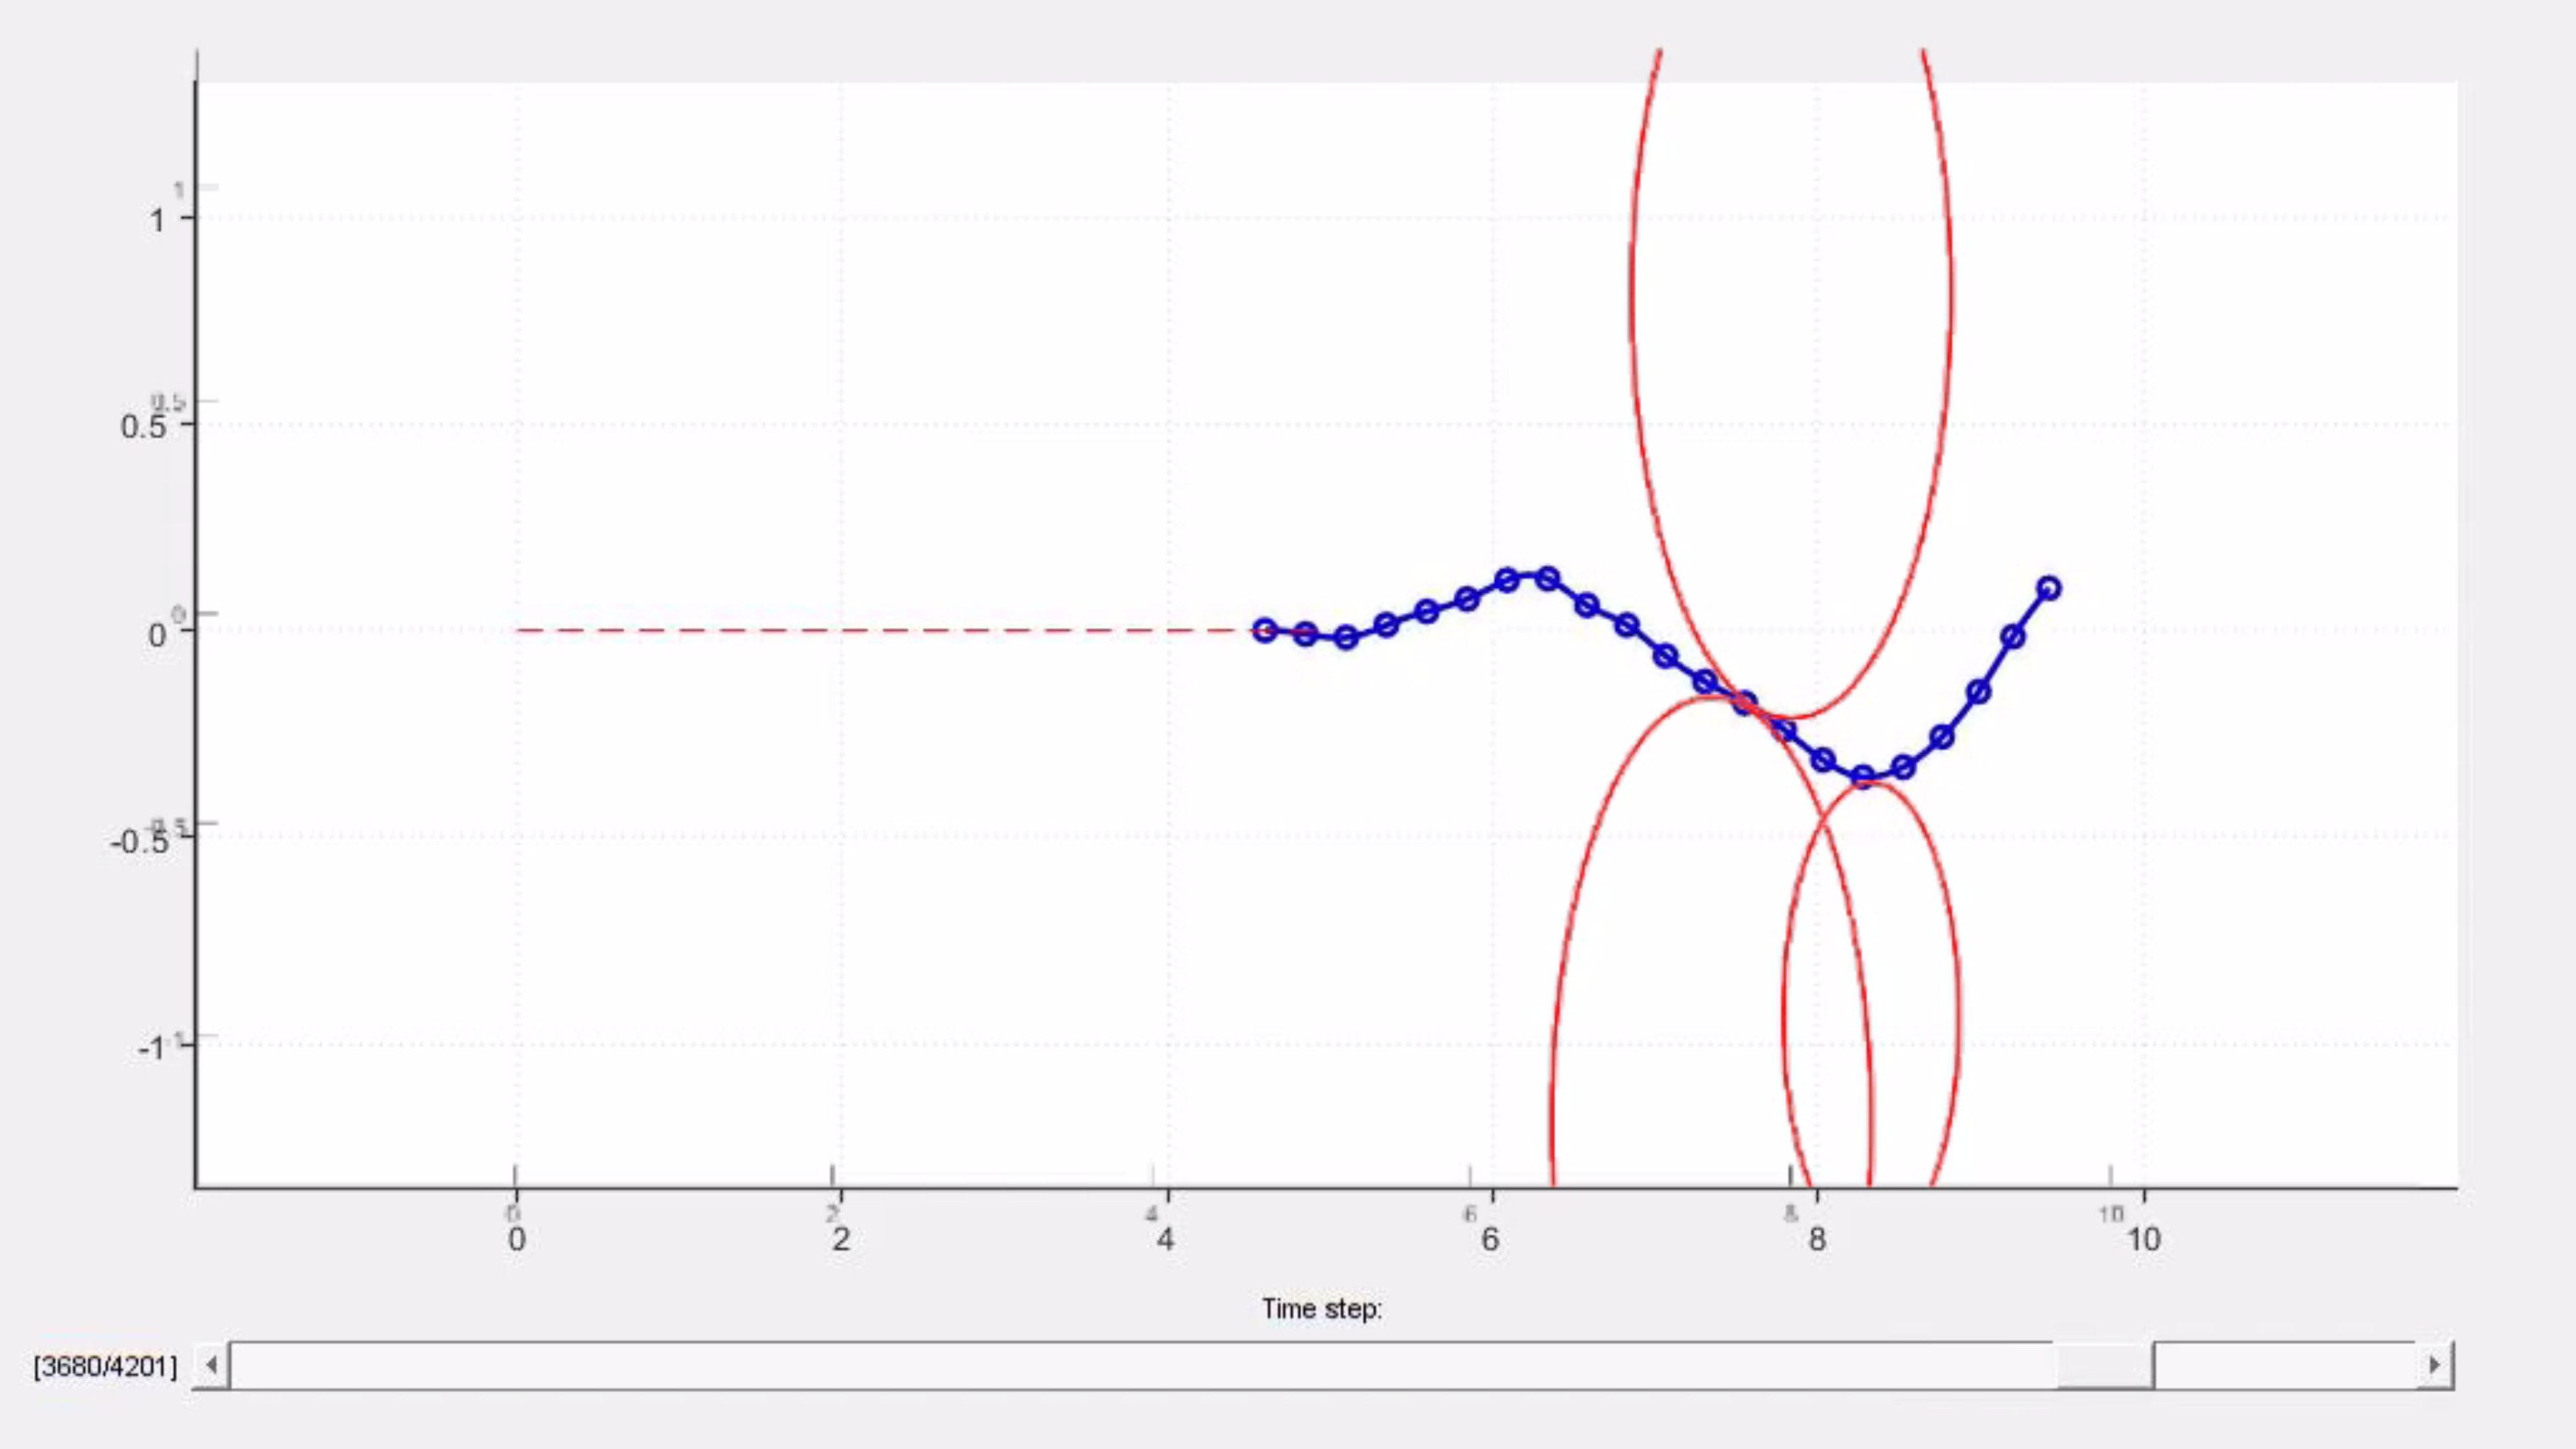
\includegraphics[width=6.27in,height=3.53in]{./media/image7.png}
		\caption{: Snapshot from simulation (before mid-sem)}
		\label{fig:_Snapshot_from_simulation_before_midsem}
	\end{Center}
\end{figure}


%%%%%%%%%%%%%%%%%%%% Figure/Image No: 7 Ends here %%%%%%%%%%%%%%%%%%%%

\par

\par

\subsection*{After Mid – Term Presentation}
\addcontentsline{toc}{subsection}{After Mid – Term Presentation}
\subsubsection*{Developing dynamic force fields}
\addcontentsline{toc}{subsubsection}{Developing dynamic force fields}
Up until now, our force fields were defined around a fixed point and were circular in shape. During the real operation however, the intestine inside the human body would deform and move due to the insertion of the medical device. It also follows that when the initial part of the large intestine is deformed, the later parts position and orientation will also change. By using fixed forcefields however, this change in the state could not be modelled appropriately.\par

Thus, instead of modelling force fields around fixed points, we modelled them around beam elements. The algorithm we developed has been outlined below:\par

\begin{itemize}
	\item Description: There are two separate bodies:\par

\begin{itemize}
	\item Body A consisting of beam elements and representing the endoscope\par

	\item Body B consisting of beam elements and representing the centreline of the intestine\par


\end{itemize}
	\item For each node of Body A, we look at its perpendicular distance to each element of Body B. In doing so, we also find the location of the base of the perpendicular dropped from the node to the element of Body B.\par

	\item As the location of nodes of Body B changes with each time step, we first determine the equation of the line passing through the two nodes. Subsequently, the perpendicular distance from each node of A is calculated. \par

	\item If the perpendicular distance is below a threshold and, if the base of the perpendicular is also with in the line segment of the element of Body B, we apply a force on the node of Body A along the perpendicular’s direction.\par

	\item The magnitude of the force is a function of  \(  \left( \text{d – l} \right)  \) . Here, d is the perpendicular distance between the node and the element while l is the threshold set by us. The equation below describes the relationship in a mathematical form. K, n are hyperparameters.\par

 \[ F~_{A}= -K \ast  \left( d- l \right) ^{n} \] \par

	\item This force is applied on the node of Body A, however and equal and opposite force also needs to be applied on the nodes of the element of Body B. For this we first must determine an appropriate ratio in which the force will be divided between the two nodes.\par

	\item The force applied on Node 1 of the element of Body B is given by:\par

\begin{Center}
 \[ F~_{B1}= F_{a}\frac{\text{"Distance between base of perpendicular and Node 2"}}{\text{"Length of the element"}} \] 
\end{Center}\par

\begin{FlushLeft}
Similarly force applied on Node 2 is:
\end{FlushLeft}\par

\begin{Center}
 \[ F~_{B2}= F_{a}\frac{\text{"Distance between base of perpendicular and Node 1"}}{\text{"Length of the element"}} \] 
\end{Center}\par

	\item The damping force is also calculated if any force is applied on the node of Body A. For this, first the component of the velocity of node A along the perpendicular to element B is calculated. Then a damping force proportional to this velocity is applied on the node of Body A in the opposite direction to its velocity.\par

	\item The reaction force on nodes of element of Body B is also applied in the same fashion as described above. The velocity of the nodes of Body B has been ignored by our model.\par

	\item We also apply the force due to friction on the node of Body A. To do this, we take several steps:\par

\begin{itemize}
	\item We first calculate the magnitude of the velocity of node of Body A along the element of Body B. \par

	\item To calculate the coefficient of friction, we use the Stick-Slip continuous friction law. Here the coefficient of friction is calculated as:\par

 \[ u =  \left\{ \begin{array}{c}
	v_{poc}\frac{ \mu _{s}}{v_{th}}\\
	u_{s}-v_{poc}\frac{ \left(  \mu _{s}- \mu _{k} \right) }{0.5\astv_{th}}\\
	 \mu _{k}\\
	\end{array} ~\begin{matrix}
v_{poc}~<~v_{th}\\
v_{th} <= v_{poc} <= 1.5\astv_{th}\\
v_{poc}~>~v_{th}\\
\end{matrix}
 \] \par

Here, the v\textsubscript{poc} is velocity at point of contact and v\textsubscript{th} is the threshold velocity.\par

	\item We are applying this force of friction only on nodes of Body A. This reaction force acting on nodes of Body B have been ignored.
\end{itemize}
\end{itemize}\par



%%%%%%%%%%%%%%%%%%%% Figure/Image No: 8 starts here %%%%%%%%%%%%%%%%%%%%

\begin{figure}[H]
\advance\leftskip 0.0in		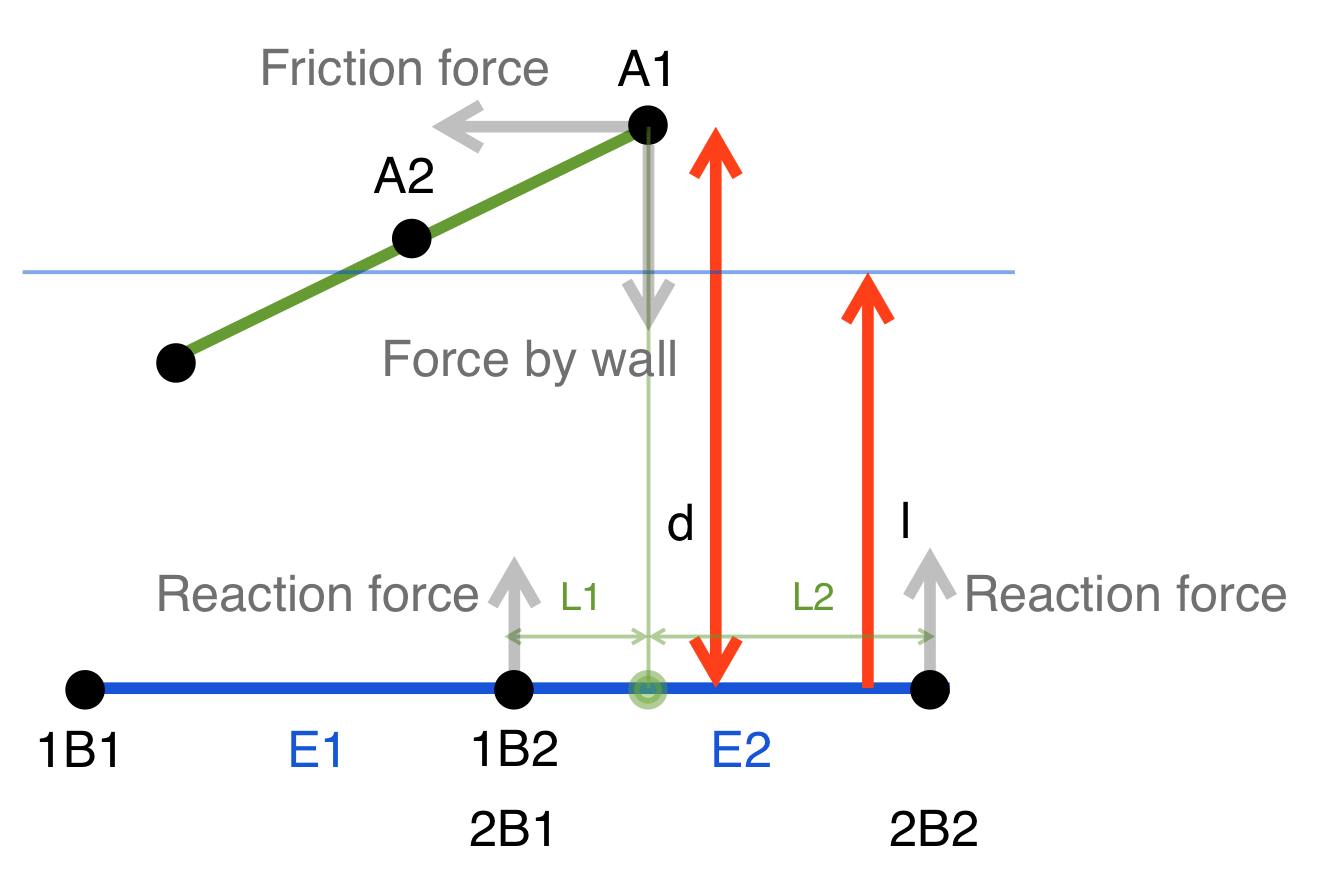
\includegraphics[width=6.27in,height=4.23in]{./media/image8.png}
\end{figure}


%%%%%%%%%%%%%%%%%%%% Figure/Image No: 8 Ends here %%%%%%%%%%%%%%%%%%%%

\subsubsection*{Mathematical description and Algorithm }
\addcontentsline{toc}{subsubsection}{Mathematical description and Algorithm }
\begin{enumerate}
	\item As input, we know the positions of A1, 2B1 $\&$  2B2. We also know  \( \dot{A1} \) . \par

	\item Let  \( \text{ax, ay} \)  be the x, y coordinates taken of A1;  \(  \left( x0, y0 \right)  \)  and  \(  \left( x1, y1 \right)  \)  be the coordinates of 2B1 and 2B2 respectively.\par

	\item We begin by calculating the equation of E1.\par

\begin{enumerate}
	\item Equation of line:  \( ax + by + c = 0 \) \par

	\item  \( a = y1 – y0 \) \par

	\item  \( b = x0 – x1 \) \par

	\item  \( c = -a\astx0 – b\asty0 \) \par


\end{enumerate}
	\item We then calculate the distance of A1 from E1 and the base at which the perpendicular from A1 will land. The base coordinates are represented as  \( \text{bx, by} \) :\par

\begin{enumerate}
	\item  \( bx =  \left(  \left( b^{2} \right) /a\astax – c – b\astay \right) / \left( a + b^{2}/a \right)  \) \par

	\item  \( by= \left( -c–a\astbx \right) /b \) \par

	\item Cases where  \( b \)  or  \( a \)  were zero were also handled.\par

	\item d was calculated by finding the distance between A1 and  \(  \left( bx, by \right)  \) \par


\end{enumerate}
	\item Similarly, L1 $\&$  L2 were also found by calculating the distance of  \(  \left( bx, by \right)  \)  from 2B1 $\&$  2B2 respectively.\par

	\item If both L1 $\&$  L2 are less than length of the element and d is greater than l, only then force is applied.\par

	\item Unit vector along the force is represented by  \(  \left( vx,vy \right)  \) \par

\begin{enumerate}
	\item  \( vx =  \left( bx – ax \right) /d \) \par

	\item  \( vy =  \left( by – ay \right) /d \) 
\end{enumerate}
\end{enumerate}\par

\subsubsection*{Adjusting model parameters}
\addcontentsline{toc}{subsubsection}{Adjusting model parameters}
Often, models like intestine and colonoscope are defined using continuum robotics using constant curvature approach. To model the colon using a centreline composed of planar beam elements is challenging because the question is: once you have defined a model, how will you represent the behaviour of the real organ. The parameters to be adjusted in our case are beam’s bending and axial stiffness and the material constant K as described in the preceding section. These parameters had to be adjusted by using the known stress strain curve of the colon wall.\par



%%%%%%%%%%%%%%%%%%%% Figure/Image No: 9 starts here %%%%%%%%%%%%%%%%%%%%

\begin{figure}[H]
	\begin{Center}
		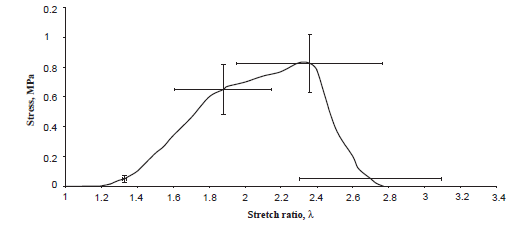
\includegraphics[width=5.28in,height=2.38in]{./media/image9.png}
		\caption{: Stress stretch curve of the large intestine}
		\label{fig:_Stress_stretch_curve_of_the_large_intestine}
	\end{Center}
\end{figure}


%%%%%%%%%%%%%%%%%%%% Figure/Image No: 9 Ends here %%%%%%%%%%%%%%%%%%%%

\par

\par

We poked a beam element of unit length representing the intestine centreline to a certain penetration depth d\textsubscript{pen}. For a given value of d\textsubscript{pen}, we can calculate the transverse force that was applied to the beam using the formula:\par

\begin{Center}
 \( F=6d_{pen}\astEI/ \left( ab\ast \left( 2a^{2}-2a \right)  \) )
\end{Center}\par

Here, a is the distance of the point (where poking is happening) from one end and b is the distance from the other (= 1-a in this case). E is the Youngs Modulus which will be obtained from the slope of the stretch-stress graph. The value of stretch is calculated using simple geometry. The new length of the beam is:\par

 \[ l^{'}=\frac{l}{\sin \theta };~tan \theta =~l/d_{pen} \] \par

The cross section is taken to be a ring such that I (moment of area)  \( I= \pi  \left( D^{4}-d^{4} \right) /64 \) \par

D and d are the outer and inner diameters of the intestinal wall respectively. This force is now transferred to the nodes of the beam element using linear interpolation (reactions on two simple supports of the beam). At various values of a and d\textsubscript{pen}, the resultant force on the nodes is obtained using SPACAR and a grid search of the three parameters (beam’s bending and axial stiffness and the material constant K) is performed till the force values are matched approximately.\par

\subsubsection*{Developing the colon model }
\addcontentsline{toc}{subsubsection}{Developing the colon model }
Human colon is modelled using 23 discrete linear elements. The mass, diameter and thickness are considered while describing the beam element and the force model.\par



%%%%%%%%%%%%%%%%%%%% Figure/Image No: 10 starts here %%%%%%%%%%%%%%%%%%%%

\begin{figure}[H]
	\begin{Center}
		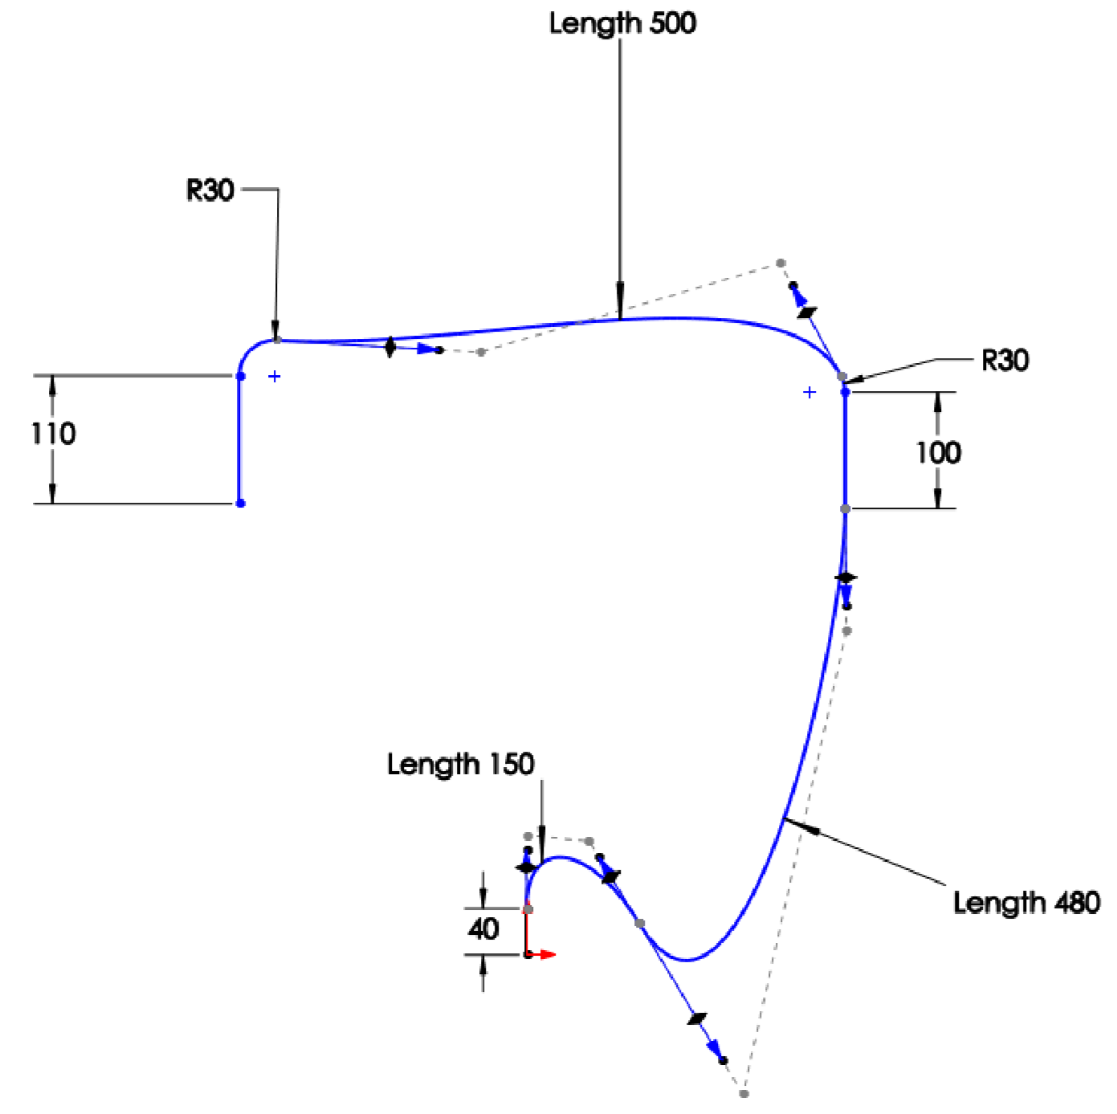
\includegraphics[width=5.09in,height=5.07in]{./media/image10.png}
	\end{Center}
\end{figure}


%%%%%%%%%%%%%%%%%%%% Figure/Image No: 10 Ends here %%%%%%%%%%%%%%%%%%%%

\begin{Center}

\end{Center}\par

\subsubsection*{Nodal interactions}
\addcontentsline{toc}{subsubsection}{Nodal interactions}
The dynamic force approach is described in detail in section 5.2.1. Force from a colon element is applicable on a node of the endoscope when the perpendicular distance between them is between l and 2l. For <l, the element is fully inside the tube and for>2l, it is assumed that it is outside the tube (and hence will not experience any force). \par



%%%%%%%%%%%%%%%%%%%% Figure/Image No: 11 starts here %%%%%%%%%%%%%%%%%%%%

\begin{figure}[H]
	\begin{Center}
		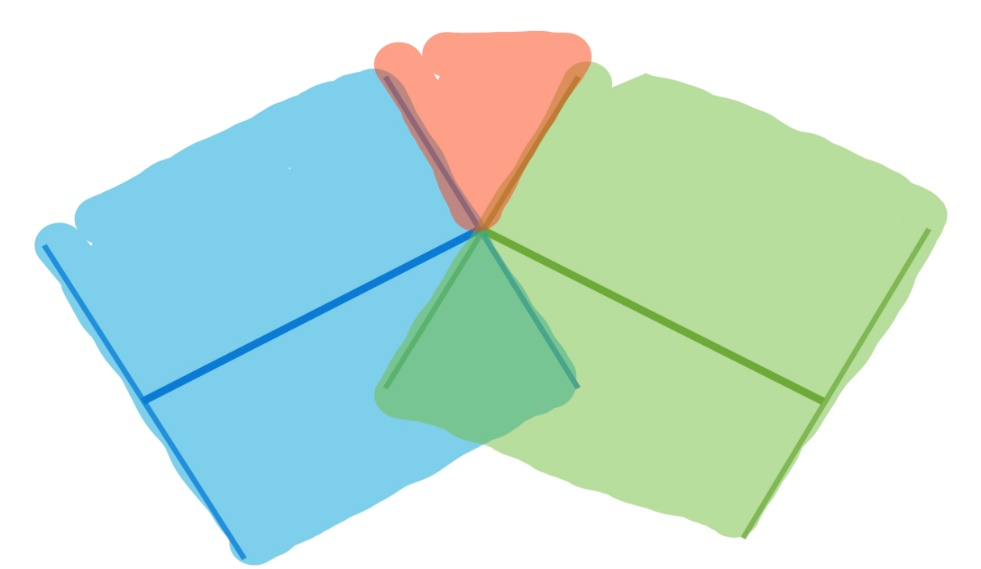
\includegraphics[width=4.46in,height=2.58in]{./media/image11.jpeg}
		\caption{0: Region of an element }
		\label{fig:0_Region_of_an_element_}
	\end{Center}
\end{figure}


%%%%%%%%%%%%%%%%%%%% Figure/Image No: 11 Ends here %%%%%%%%%%%%%%%%%%%%

\par

\par

However, there are some corner cases which may be left unaccounted for. The elements being discrete, some nodes may not lie in the region of any of the elements. Region of an element is shown in the diagram below as the blue and green shaded area. For such nodes (i.e. in the centre red region of the figure) of the endoscope, we simply calculate the force based on its interaction with the node of the colon which is closest to it.\par


\vspace{\baselineskip}
\subsection*{Simulation Details}
\addcontentsline{toc}{subsection}{Simulation Details}
\subsubsection*{Endoscope}
\addcontentsline{toc}{subsubsection}{Endoscope}
\par



%%%%%%%%%%%%%%%%%%%% Table No: 4 starts here %%%%%%%%%%%%%%%%%%%%


\begin{table}[H]
 			\centering
\begin{tabular}{p{2.91in}p{2.91in}}
\hline
%row no:1
\multicolumn{1}{|p{2.91in}}{Type of Elements} & 
\multicolumn{1}{|p{2.91in}|}{Planar Beam} \\
\hhline{--}
%row no:2
\multicolumn{1}{|p{2.91in}}{Number of Elements} & 
\multicolumn{1}{|p{2.91in}|}{10} \\
\hhline{--}
%row no:3
\multicolumn{1}{|p{2.91in}}{Length} & 
\multicolumn{1}{|p{2.91in}|}{0.6 m} \\
\hhline{--}
%row no:4
\multicolumn{1}{|p{2.91in}}{Mass per unit length} & 
\multicolumn{1}{|p{2.91in}|}{0.001532 kg/m} \\
\hhline{--}
%row no:5
\multicolumn{1}{|p{2.91in}}{Rotational Inertia J} & 
\multicolumn{1}{|p{2.91in}|}{0.00000000002393 kg-m\textsuperscript{2}} \\
\hhline{--}
%row no:6
\multicolumn{1}{|p{2.91in}}{Axial Stiffness (EA)} & 
\multicolumn{1}{|p{2.91in}|}{700 N/m} \\
\hhline{--}
%row no:7
\multicolumn{1}{|p{2.91in}}{Bending Stiffness (EI)} & 
\multicolumn{1}{|p{2.91in}|}{0.003 N/m} \\
\hhline{--}
%row no:8
\multicolumn{1}{|p{2.91in}}{Longitudinal Damping} & 
\multicolumn{1}{|p{2.91in}|}{0.000001 N-s/m} \\
\hhline{--}
%row no:9
\multicolumn{1}{|p{2.91in}}{Bending Damping} & 
\multicolumn{1}{|p{2.91in}|}{{\fontsize{10pt}{12.0pt}\selectfont  }0.00001{\fontsize{10pt}{12.0pt}\selectfont  }N-s/m} \\
\hhline{--}

\end{tabular}\caption{: Properties of the colon}
\label{tab:: Properties of the colon}

 \end{table}


%%%%%%%%%%%%%%%%%%%% Table No: 4 ends here %%%%%%%%%%%%%%%%%%%%


\vspace{\baselineskip}
\subsubsection*{Colon}
\addcontentsline{toc}{subsubsection}{Colon}
\par



%%%%%%%%%%%%%%%%%%%% Table No: 5 starts here %%%%%%%%%%%%%%%%%%%%


\begin{table}[H]
 			\centering
\begin{tabular}{p{2.91in}p{2.91in}}
\hline
%row no:1
\multicolumn{1}{|p{2.91in}}{Type of Elements} & 
\multicolumn{1}{|p{2.91in}|}{Planar Beam} \\
\hhline{--}
%row no:2
\multicolumn{1}{|p{2.91in}}{Number of Elements} & 
\multicolumn{1}{|p{2.91in}|}{23} \\
\hhline{--}
%row no:3
\multicolumn{1}{|p{2.91in}}{Length} & 
\multicolumn{1}{|p{2.91in}|}{1.38 m} \\
\hhline{--}
%row no:4
\multicolumn{1}{|p{2.91in}}{Mass per unit length} & 
\multicolumn{1}{|p{2.91in}|}{ \tabto{0.97in} 0.08532 kg/m} \\
\hhline{--}
%row no:5
\multicolumn{1}{|p{2.91in}}{Rotational Inertia J} & 
\multicolumn{1}{|p{2.91in}|}{0.00008393 kg-m\textsuperscript{2}} \\
\hhline{--}
%row no:6
\multicolumn{1}{|p{2.91in}}{Axial Stiffness (EA)} & 
\multicolumn{1}{|p{2.91in}|}{500 N/m} \\
\hhline{--}
%row no:7
\multicolumn{1}{|p{2.91in}}{Bending Stiffness (EI)} & 
\multicolumn{1}{|p{2.91in}|}{0.0025 N/m} \\
\hhline{--}
%row no:8
\multicolumn{1}{|p{2.91in}}{Longitudinal Damping} & 
\multicolumn{1}{|p{2.91in}|}{0.000001 N-s/m} \\
\hhline{--}
%row no:9
\multicolumn{1}{|p{2.91in}}{Bending Damping} & 
\multicolumn{1}{|p{2.91in}|}{{\fontsize{10pt}{12.0pt}\selectfont  }0.00001{\fontsize{10pt}{12.0pt}\selectfont  }N-s/m} \\
\hhline{--}
%row no:10
\multicolumn{1}{|p{2.91in}}{Inner Diameter} & 
\multicolumn{1}{|p{2.91in}|}{\Centering 30 mm} \\
\hhline{--}
%row no:11
\multicolumn{1}{|p{2.91in}}{Thickness} & 
\multicolumn{1}{|p{2.91in}|}{\Centering 2 mm} \\
\hhline{--}
%row no:12
\multicolumn{1}{|p{2.91in}}{Friction Coefficient} & 
\multicolumn{1}{|p{2.91in}|}{\Centering 0.4} \\
\hhline{--}

\end{tabular}\caption{gure 11: Snapshot from simulation}
\label{tab:gure 11: Snapshot from simulation}

 \end{table}


%%%%%%%%%%%%%%%%%%%% Table No: 5 ends here %%%%%%%%%%%%%%%%%%%%


\vspace{\baselineskip}


%%%%%%%%%%%%%%%%%%%% Figure/Image No: 12 starts here %%%%%%%%%%%%%%%%%%%%

\begin{figure}[H]
	\begin{Center}
		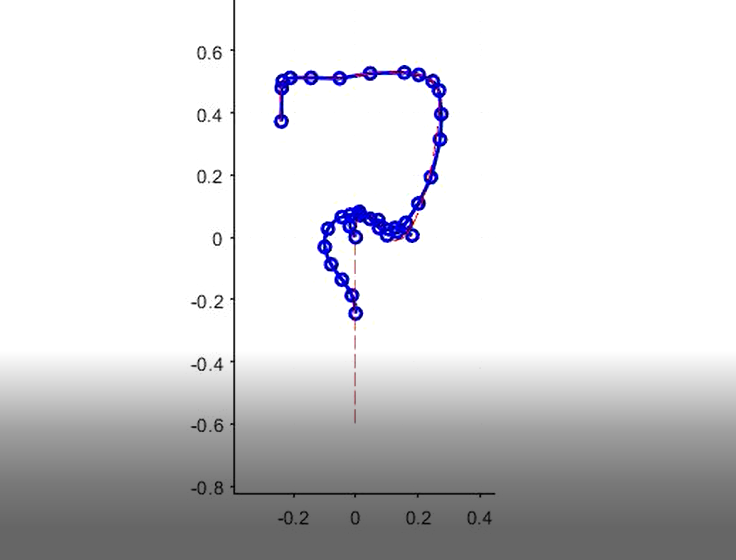
\includegraphics[width=4.4in,height=4.36in]{./media/image12.png}
		\caption{1: Snapshot from simulation}
		\label{fig:1_Snapshot_from_simulation}
	\end{Center}
\end{figure}


%%%%%%%%%%%%%%%%%%%% Figure/Image No: 12 Ends here %%%%%%%%%%%%%%%%%%%%

\par

\par

\begin{FlushLeft}
The simulation is carried out for 5 seconds in 20,000 timesteps.

 %%%%%%%%%%%%  Starting New Page here %%%%%%%%%%%%%%

\newpage

\end{FlushLeft}\par

\section*{Conclusion}
\addcontentsline{toc}{section}{Conclusion}
In this project, we have introduced a novel method to carry out the simulation of two soft deformable bodies using force fields. For doing so, we had to develop algorithms that find distances of all nodes of one body from the elements or nodes of the second body as well as the magnitude and direction of force, if so required, to be applied. We make the use of the software SPACAR to accurately simulate the deformations and movement of the beam elements that have been used as building blocks for both bodies that are interacting.\par

A standout feature of the framework developed by us is that it can be applied in multiple places. The user only needs to input the coordinates of the nodes of both the bodies to start off. We have also developed another algorithm discussed in section 5.2.2 where the user can optimise parameters of the beam element to match closely with the behaviour seen in real life for a very simple case. This information is then used to model the behaviour for more complicated cases. Another feature of our framework is the need of very less computation power in comparison to other the FEA methods. Once the simulation has been carried out, our model allows the user to view the simulation easily at each time step. Apart from the visual orientation of all bodies, the framework also provides information on the amount of force and stress that is being applied on the body.\par

While our framework has been able to model the expected behaviour very well for the simple situation, we do not have any benchmark to compare its performance of simulations carried out on the large intestine. Our model is also currently limited to two dimensions. A separate and more evolved algorithm will be required for carrying out these simulations in three dimensions. Thus, our framework is an important first step in the modelling of soft bodies and using analytical solutions of beam elements to study their interaction. However, it is far from being complete and shall require extensive validation and refinement before it can be used as a trustable source of information.\par



 %%%%%%%%%%%%  Starting New Page here %%%%%%%%%%%%%%

\newpage

\vspace{\baselineskip}\printbibliography

\printbibliography
\end{document}